\chapter{State \& parameter estimation}
\label{chapter:state-parameter-estimation}

\section{Motivation for state and parameter estimation}
The flight data used in this report comes from an F-16 experiment that measured the aircraft's angle of attack ($\alpha_m$), angle of sideslip ($\beta_m$) and velocity ($V_m$). However, it is known that the angle of attack measurements are biased due to an upwash ($C_{\alpha_{up}}$) that occurs at the location of the sensors vane. The angle of sideslip and velocity, on the other hand, are not biased.

A biased result would be obtained if the flight data experiment were to be directly used to construct a model. The bias contained in the angle of attack measurements would be passed into the model's predictions. A solution to this problem is to use state estimation to improve the quality of the experimental data. Using a Kalman Filter (KF), the bias in the angle of attack can be determined, and the aircraft states can be reconstructed. This process extracts the influences that are not part of the actual aircraft behaviour from the measured states. 

The reconstructed measurement data is suitable for building an aircraft model. This process, however, requires a selection of parameters that define the model. An optimal model can be created by choosing the parameters that minimise the error of the predictions. For example, in a polynomial model, it is needed to determine the value of its coefficients. Determining those coefficients is a type of parameter estimation.

Together, state and parameter estimation allow the creation of an unbiased and optimal model. The state estimation process ensures that bias-free data is passed to the construction of the model. The parameter estimation ensures optimal use of the available data to determine the model coefficients.


\section{Model description}
The first step in the state estimation process is determining how the states, inputs and noise influence the model's states and outputs. Only with that defined the KF can be constructed. For the studied F-16 flight data, four states are considered - the three contributions of the speed vector and the unknown upwash coefficient (the coefficient that will be determined from the KF). The aircraft state and measurement vectors are described in \autoref{eq:state-vector} and \autoref{eq:measurement-vector}, respectively. 

\begin{equation}\label{eq:state-vector}
  x_k = 
	\begin{bmatrix}
	u & v & w & C_{\alpha_{up}}
	\end{bmatrix}^T
\end{equation}

\begin{equation}\label{eq:measurement-vector}
  z_k = 
	\begin{bmatrix}
	\alpha_m & \beta_m & V_m
	\end{bmatrix}^T
\end{equation}


The input vector, shown in \autoref{eq:input-vector}, is the linear acceleration vector obtained from an unbiased accelerometer sampled every \SI{0.01}{\second}.

\begin{equation}\label{eq:input-vector}
  u_k =
	\begin{bmatrix}
	\dot{u} & \dot{v} & \dot{w}
	\end{bmatrix}^T
\end{equation}

The input vector is considered to be unbiased. Also the system dynamics are trivial and only depends on the system inputs. Therefore the system dynamic equation is defined by:

\begin{equation*}
  \dot{x}_k =
	\begin{bmatrix}
	1 & 0 & 0\\
	0 & 1 & 0\\
	0 & 0 & 1\\
	0 & 0 & 0\\
	\end{bmatrix}
	u_k
	+
	\begin{bmatrix}
	w_u \\
	w_v \\
	w_w \\
	w_c \\
	\end{bmatrix}
\end{equation*}

The observation equation is non-linear and is described by the relation:

\begin{equation*}
	z_k =
	\underbrace{
	\begin{bmatrix}
	tan^{-1}(\frac{w}{u})(1+C_{\alpha_{up}}) \\
	tan^{-1}(\frac{v}{\sqrt{u^2+w^2}}) \\
	\sqrt{u^2+v^2+w^2}
	\end{bmatrix}
	}_{h(x(t), u(t), t)}
	+
	\begin{bmatrix}
	v_\alpha \\
	v_\beta \\
	v_V
	\end{bmatrix}
\end{equation*}


In the KF, the observation equation can only be used after being linearised. That is done by generating the Jacobian ($H_x$) of the observation matrix $h$, which is shown in \autoref{eq:jacobian}.

\begin{equation}\label{eq:jacobian}
	H_x = \frac{\delta}{\delta x}h =
\begin{bmatrix}
\frac{-w}{u^2+w^2}(1+C_{\alpha_{up}}) & 0 & \frac{u}{u^2+w^2}(1+C_{\alpha_{up}}) & tan^{-1}(\frac{w}{u}) \\

\frac{-uv}{(u^2+v^2+w^2)\sqrt{u^2+w^2}} & \frac{\sqrt{u^2+w^2}}{(u^2+v^2+w^2)} & \frac{-vw}{(u^2+v^2+w^2)\sqrt{u^2+w^2}} & 0 \\
\frac{u}{\sqrt{u^2+v^2+w^2}} & \frac{v}{\sqrt{u^2+v^2+w^2}} & \frac{w}{\sqrt{u^2+v^2+w^2}} & 0
\end{bmatrix}  x_k
\end{equation}

\section{State estimation with an Iterated Extended Kalman Filter}
The KF built to perform the state estimation is the Iterated Extended Kalman Filter. This filter was selected for two reasons. (1) The observation equation is non-linear; therefore, the Linear Kalman Filter cannot be used. (2) The IEKF ensures global convergence, which is not the case for the Extended Kalman Filter (EKF)

Linearising the observation equation inevitably introduces errors into the model. The IEKF reduces this error by iterating and improving the linearization point for each loop of the KF. That means that in one loop of the IEKF, the errors due to the model linearization are reduced, making the filter converge faster than the EKF and behave closer to a linear KF. In practice, this filter makes more efficient use of the available observation data, which is not wasted to correct the linearization errors.


\todo{Add summary of KF steps}

With the constructed Kalman Filter, the upwash coefficient is estimated. \autoref{fig:upwash} shows how the coefficient changes through the iterations and how it converges to 0.23. The convergence of this coefficient is an indication that the KF has converged.

\begin{figure}[h]\centering
  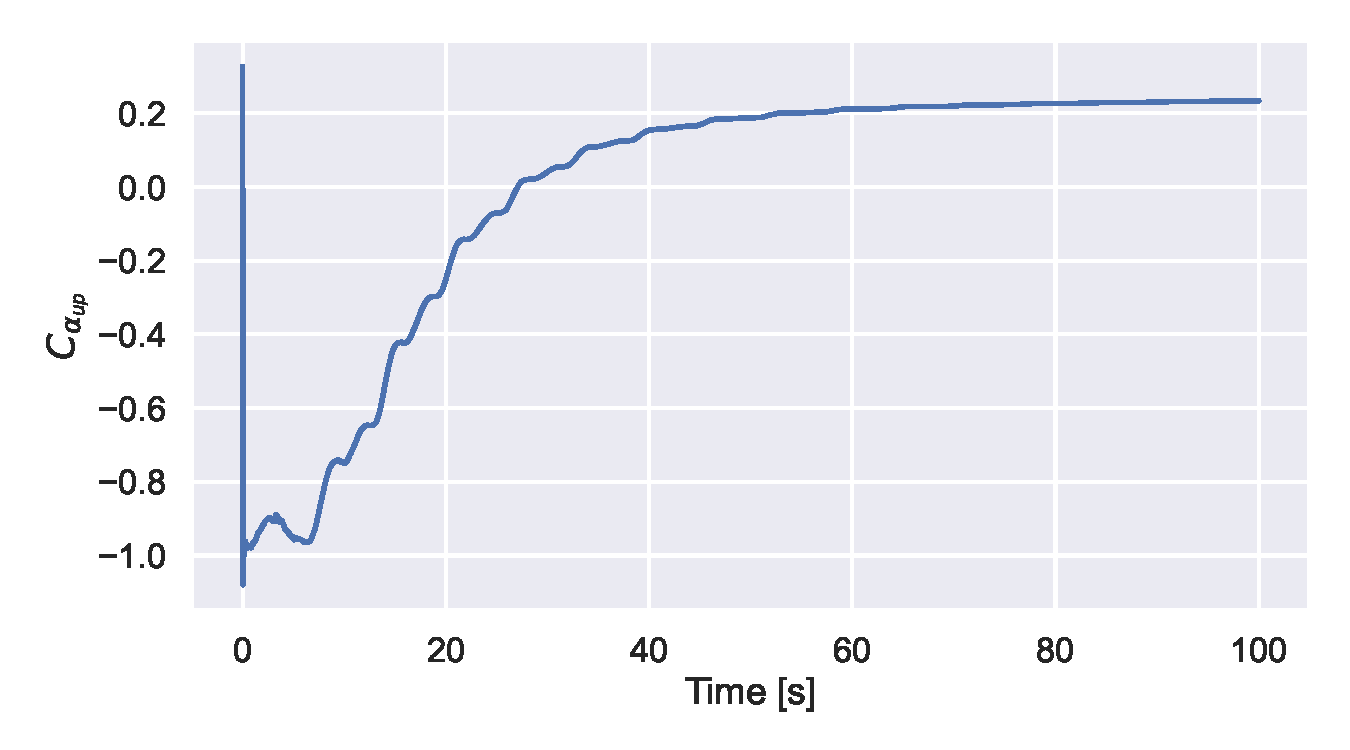
\includegraphics[width=0.8\textwidth]{figures/state_estimation_wash.pdf}
  \caption{Estimated $C_{\alpha_{up}}$ from the IEKF.}
  \label{fig:upwash}

\end{figure}

The relation between the measured and true angle of attack is known and described by \autoref{eq:alpha-relation}. The true angle of attack can be derived using the estimated $C_{\alpha_{up}}$. \autoref{fig:alpha-comparison} shows the difference between the $\alpha_m$ and $\alpha_{true}$. This process completes the remotion of the bias from the angle of attack. Only after that are the measurements of this state propitious for the model construction. The model output is shown in \autoref{fig:model-output}\todo{write about output}

\begin{figure}[H]
\centering
  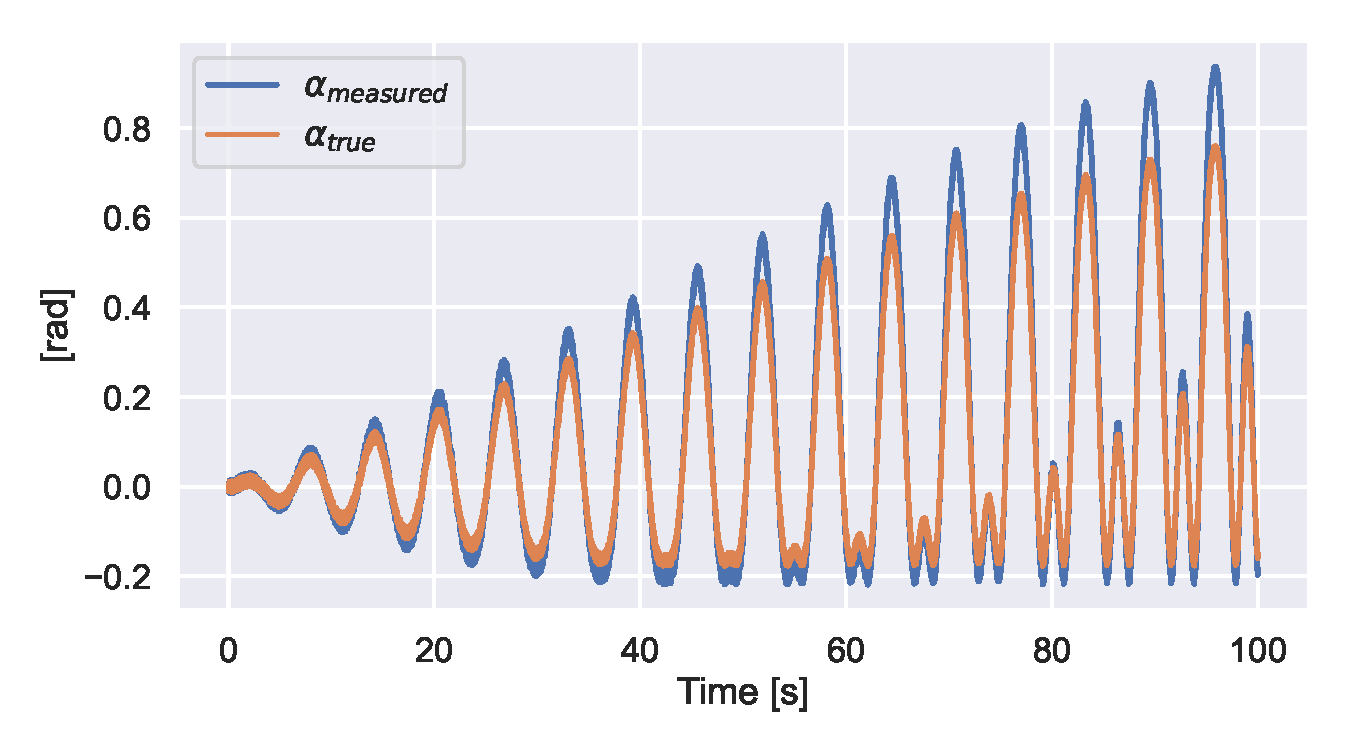
\includegraphics[width=0.8\textwidth]{figures/state_estimation_alpha.pdf}
  \caption{Comparison between measured and true angle of attack.}
  \label{fig:alpha-comparison}
\end{figure}

\begin{figure}[h]
\centering
  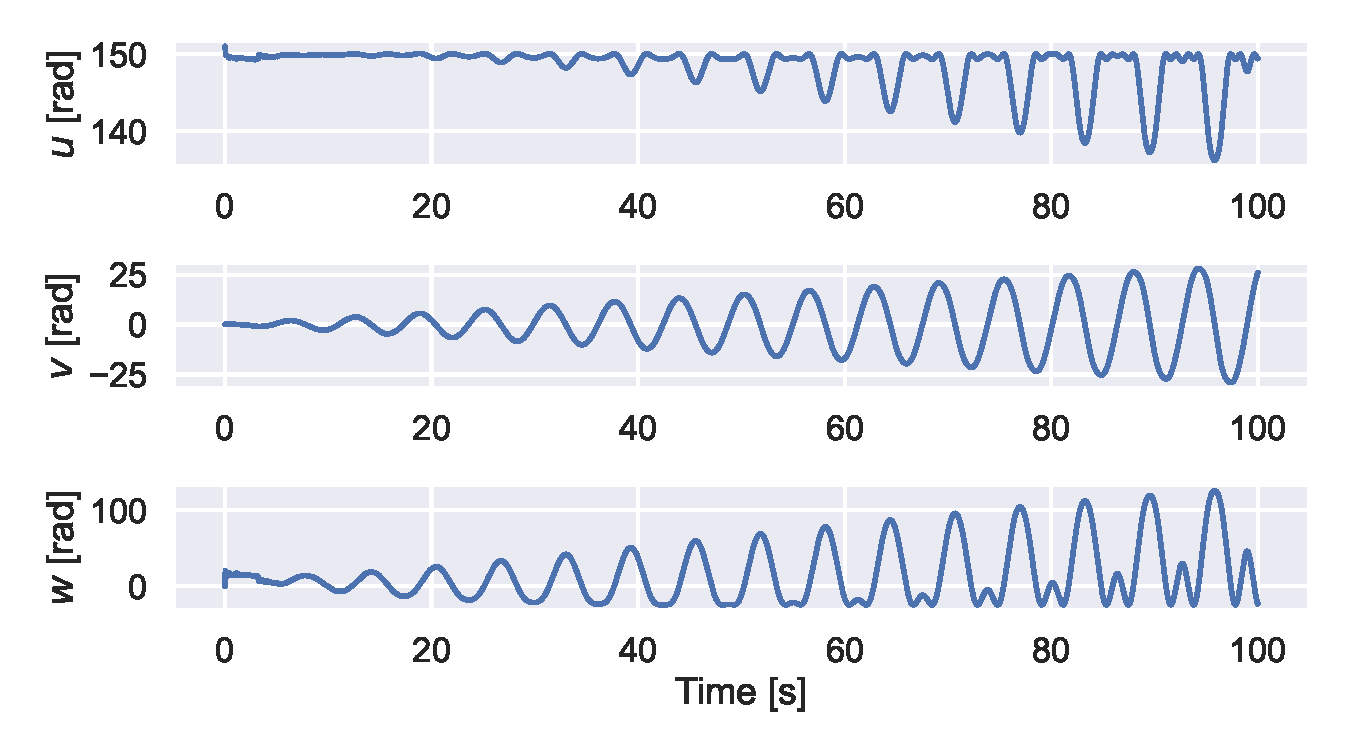
\includegraphics[width=0.8\textwidth]{figures/state_estimation_output.pdf}
  \caption{Estimated aircraft output.}
  \label{fig:model-output}
\end{figure}


\section{Parameter estimation with an ordinary least squares regression}
The IEKF reconstructed F-16 flight data, making it ideal for constructing a model for the aircraft. This report makes use of a polynomial structure to model this data. The model parameters (i.e., the polynomial coefficients) are determined by implementing an ordinary least squares (OLS) estimator. 

\begin{equation}\label{eq:alpha-relation}
  \alpha_{true} = \frac{\alpha_m}{1+C_{\alpha_{up}}}
\end{equation}

For each angle of attack true value (value with removed bias) and sideslip angle, a measurement of the moment coefficient is available $C_m$. Therefore, a model with $\alpha_{true}$ and $\beta_m$ and input and $C_m$ as output can be constructed. Therefore, the described model is defined by \autoref{eq:cm-equation}. In this equation, $A(x)$ is the regression matrix, $\theta$ is the parameters vector, and $\epsilon$ is the model error. 

\begin{align}\label{eq:cm-equation}
  c_m &= A(\alpha , \beta)\cdot \theta + \epsilon \\
   &= \begin{bmatrix}
1 &\alpha & \beta & \alpha^2 & \beta^2 & \alpha\cdot\beta & \cdots & \beta^M
\end{bmatrix}\cdot \theta + \epsilon
\end{align}


The parameter estimation problem is solved by determining the value os of the parameter vector $\theta$ such that a cost function is minimised. For the F-16 model, an ordinary least squares estimator was used with a quadratic cost function, as shown in \autoref{eq:cost-function}. 

\begin{equation}\label{eq:cost-function}
	J(x, \theta) = \sum^N_{i=1}(y_i-A(x_i)\cdot\theta)^2
\end{equation}

From \todo{cite presentation}, it is known that the best estimation of $\theta$ comes from the relation:
\begin{equation*}
	\bar{\theta}=(A^T(x)\cdot A(x))^{-1}A^T(x)\cdot y
\end{equation*}

The order of the polynomial used in the linear regression is a model hyper-parameters that can define the performance of the estimations. For a polynomial of order 2, it was found that the $c_m$ can be determined with  \autoref{}.

\begin{equation}
	C_{m_{estimated}} = -0.064 + 0.020 \alpha + 0.003 \beta -0.001 \alpha^2 +0.158 \beta^2 -0.030 \alpha \beta
\end{equation}

The variance of the coefficients was determined by \autoref{eq:variance-pol}. In this equation, $\epsilon$ is the residuals vector, $n$ is the number of measurements, and $k$ is the number of regressor terms. The variance of each coefficient of the second order polynomial are provided in \todo{add table}.

\begin{equation}\label{eq:variance-pol}
	Var\{\hat{\theta}\} = diag(\frac{\epsilon^T\epsilon}{n-k}(A^T(x)\cdot A(x))^{-1})
\end{equation}

For different polynomial orders, different models are determined. \autoref{fig:rms-pol} shows the root mean squared (RMS) of the residuals for each polynomial order. Increasing the polynomial order, the estimation error of the training dataset reduces. However, for the validation dataset, the error increases for orders higher than 3. That happens because increasing the complexity of the model by adding more coefficients results in an overfit of the training data. Therefore, the model cannot generalise the solution for data it has not seen during fitting. 

\begin{figure}[h]
\centering
  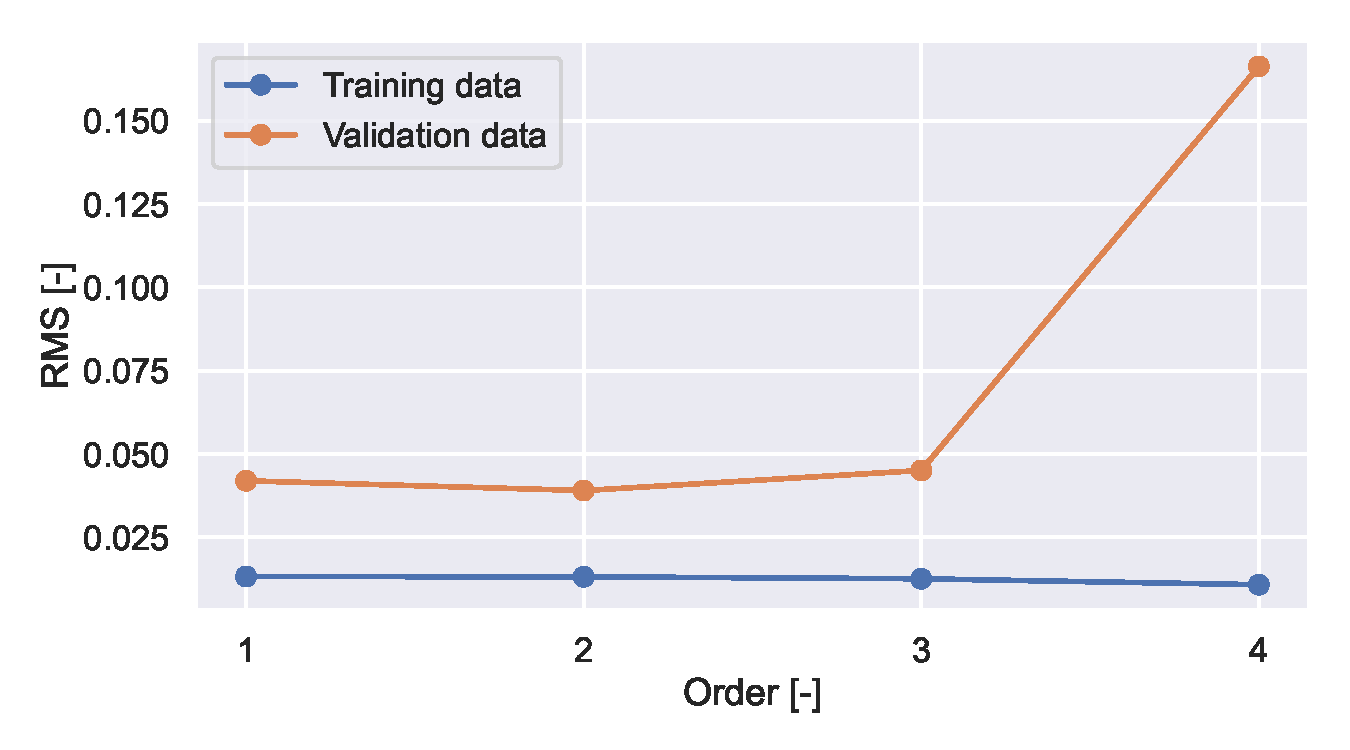
\includegraphics[width=0.8\textwidth]{figures/parameter_estimation_mse}
  \caption{Root mean squared error per polynomial order}
  \label{fig:rms-pol}
\end{figure}

Another reason for the reduction in performance in the validation dataset is that the training data does not overlap entirely with the measured data. In \autoref{fig:training-validation}, it can be seen that part of the validation data is not in an area where the model was trained. 

\begin{figure}[h]
\centering
  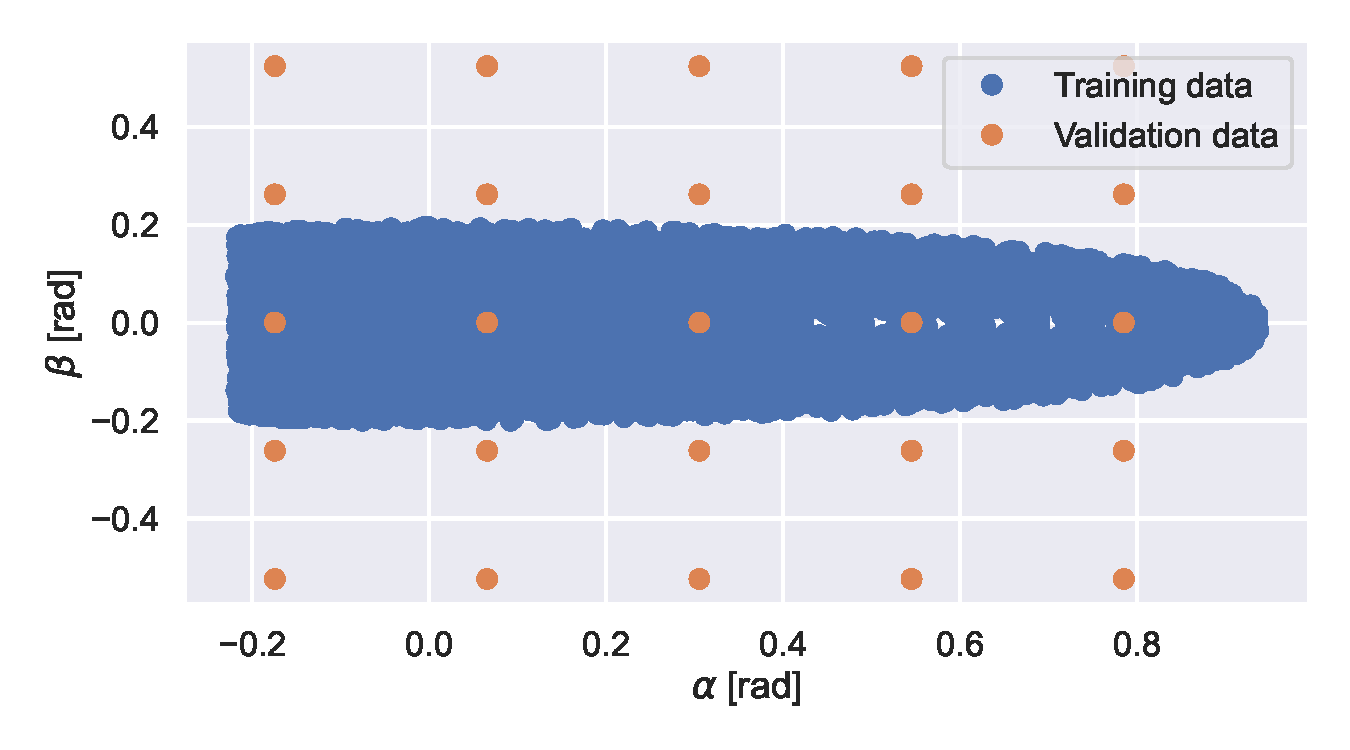
\includegraphics[width=0.8\textwidth]{figures/parameter_estimation_domain}
  \caption{Training and validation data span.}
  \label{fig:training-validation}
\end{figure}


